\documentclass[12pt]{article}

\usepackage{german}
\usepackage{geometry}
\usepackage[onehalfspacing]{setspace}

\geometry{
    left=3cm,
    right=3cm,
    top=2.5cm,
    bottom=2.5cm
}

\usepackage{listings}
\usepackage{xcolor}

\usepackage{amsmath}
\usepackage{amssymb}

\usepackage{url}

\setlength{\emergencystretch}{15pt}

\lstset{
    tabsize = 4, %% set tab space width
    showstringspaces = false, %% prevent space marking in strings, string is defined as the text that is generally printed directly to the console
    numbers = left, %% display line numbers on the left
    commentstyle = \color{green}, %% set comment color
    keywordstyle = \color{blue}, %% set keyword color
    stringstyle = \color{red}, %% set string color
    rulecolor = \color{black}, %% set frame color to avoid being affected by text color
    basicstyle = \small \ttfamily , %% set listing font and size
    breaklines = true, %% enable line breaking
    numberstyle = \tiny,
}

\title{Numerisches finden von Nullstellen - Implementierung in Java}
\author{Jakob Rzeppa}

\begin{document}
\begin{titlepage}
	\centering
    {\huge IGSFF LOGO TODO\par}
	{Grünewaldstraße 12a - 38104 Braunschweig - T. 470 5850\par}
	\vspace{1cm}
	{\underline{Seminarfach:}\par}
	\vspace{1cm}
    {\large Facharbeit des Schülers \textit{Jakob Rzeppa} \par mit dem Thema: \par}
    \vspace{1.5cm}
	{\huge Numerisches finden von Nullstellen - Implementierung in Java\par}
	\vspace{2cm}
\end{titlepage}

\tableofcontents

\section{Einleitung}

\subsection{Problemstellung}
Mithilfe von Nullstellen kann man viel über den Verlauf einer Polynomfunktion herrausfinden. In der Schule lernt man mit der PQ-Formel oder ABC-Formel das Finden von Nullstellen zweiten Grades. Manchmal werden außerdem kubische Funktionen und deren Nullstellen betrachtet, jedoch wird das algebraische finden von Nullstellen ab dem vierten Grad meist unmöglich. Für diese muss meist auf ein anderen Teilbereich der Mathematik zurückgegriffen werden: die Numerik. In der Numerik versucht man durch Algorithmen und Annärhungen Nullstellen möglichst genau zu bestimmen. Händisch kann dies sehr lange dauern, jedoch kann mit Computern dieser Prozess extrem beschleunigt werden. Doch wie kann man Nullstellen von Polynomen mithilfe des Computers approximieren?

\subsection{Wie bin ich auf das Thema gekommen?}
Seid ich das erste mal Nullstellenberechnung mithilfe der PQ-Formel hatte hat es mich interessiert, wie man die Nullstellen von Polynomen mit einem Grad größer als zwei findet. Als Herr Heydecke mir das Thema Numerisches lösen von linearen Gleichungssystemen vorgeschlagen hatte habe ich mich an mein Interesse für das Lösen der Nullstellen von Polynomfunktionen erinnert und entschieden dieses Thema für die Facharbeit zu wählen.

\subsection{Herangehensweise}
Um die Problemfrage zu lösen werde ich zuerst unterschiedliche Verfahren vergleichen. Von diesen werde ich das Geeingnetste näher betrachten. Daraufhin werde ich die gewählte Methode implementieren. 

\section{Vergleich von Methoden}
In der Numerik gibt es viele verschiedene Verfahren für die Nullstellenberechnung. Das meist bekannteste ist das Newton-Methode\footnote{
    Prof. Dr. Bernd Engelmann: Numerische Mathematik, 2.4 Das Newton-Verfahren und seine Abkömmlinge (S.24)
} oder das Bisektionsverfahren bzw. der Zwischenwertsatz\footnote{
    mathe-online.at: Zwischenwertsatz und Bisektionsverfahren, URL: \url{https://www.mathe-online.at/nml/materialien/innsbruck/bisektion/Bisektion.pdf}
}. Beide Methoden sind jedoch nur für das Finden einer Nullstelle geeignet.\\
\\
Wenn man alle Nullstellen finden möchte muss man komplexere Verfahren in betracht ziehen. Dabei bieten sich Weiterentwicklungen der Newton-Methode wie die Weierstraß-Iteration, das Aberth-Ehrlich-Verfahren, das Trennkreisverfahren oder das Newton-Horner-Verfahren an. Dabei finden die drei ersten Methoden die Nullstellen simultan, während das Newton-Horner-Verfahren die Nullstellen nacheinander findet. Aus diesem Grund ist das Newton-Horner-Verfahren meist langsamer als die anderen Methoden und wird nicht weiter behandelt. Das Trennkreisverfahren basiert auf komplexeren mathematischen Grundlagen als die Weierstraß-Iteration und das Aberth-Ehrlich-Verfahren und ist deshalb schwieriger zu implementieren. Zuletzt bleibt die Entscheidung zwischen der Weierstraß-Iteration und dem Aberth-Ehrlich-Verfahren. Beide Verfahren sind sich sehr ähnlich. Das Aberth-Ehrlich-Verfahren ist etwas schneller als die Weierstraß-Iteration, benutzt jedoch die Ableitung des Polynoms und ist ein wenig komplexer. Aus diesem Grund wird die Weierstraß-Iteration implementiert. Diese ist nicht das schnellste Verfahren, jedoch kann sie gut Implementiert werden und ist besser als die anderen Verfahren zu beschreiben.
%TODO Fußnoten

\section{Weierstraß-Iteration}
\subsection{Funktionsweise}
\subsubsection{Bedingungen}
Für die Weierstraß-Iteration muss ein normiertes univariates Polynom der Form $p(x) = x^n + a_{n-1} x^{n-1} + \dots + a_1 x + a_0$ gegeben sein. Der Grad des Polynoms $n$ muss größer als oder gleich zwei sein.\footnote{
    vgl. Wikipedia: Weierstraß-(Durand-Kerner)-Verfahren, URL: \url{https://de.wikipedia.org/wiki/Weierstraß-(Durand-Kerner)-Verfahren} (Zuletzt eingesehen am 29.10.2023)
    \label{ftn:Wikipedia-Weierstraß-Methode}
}

\subsubsection{Gleichungen für die Weierstraß-Iteration}
Bei der Weierstraß-Iteration wird mit jeder Iteration jede Nullstelle etwas genauer. Dafür werden $n$ Gleichungen für die $n$ Nullstellen\footnote{Eine Funktion $n$ten Grades hat nach dem Fundamentalsatz der Algebra genau $n$ komplexe Nullstellen.} $z_n;z_{n-1};\dots;z_1$ gebildet. Über diese wird, bis das Endkriterium erreicht ist, iteriert. Dabei ist $i$ die Anzahl der Iterationen und wird pro Iteration um 1 inkrementiert.
\[z_n^{(i+1)} = z_n^{(i)} - \frac{p(z_n^{(i)})}{\prod_{j=1;j\neq n}^{n}(z_n^{(i)}-z_j^{(i)})}\]
\[z_{n-1}^{(i+1)} = z_{n-1}^{(i)} - \frac{p(z_{n-1}^{(i)})}{\prod_{j=1;j\neq n-1}^{n}(z_{n-1}^{(i)}-z_j^{(i)})}\]
\vspace{0.25mm}
\[\dots\]
\[z_{1}^{(i+1)} = z_1^{(i)} - \frac{p(z_{1}^{(i)})}{\prod_{j=1;j\neq 1}^{n}(z_{1}^{(i)}-z_j^{(i)})}\]
\subsubsection{Startpunkte}
Zunächst müssen alle Startpunkte $z_n^{(0)};z_{n-1}^{(0)};\dots;z_1^{(0)} \in \mathbb{C}$ gesetzt werden. Diese können beliebig gewählt werden. Es muss jedoch beachtet werden, dass Startpunkte für komplexe Nullstellen einen imaginären Teil ungleich Null haben müssen. Außerdem müssen alle Startpunkte unterschiedlich sein, damit bei der ersten Iteration nicht durch Null dividiert wird. Denn bei der Gleichung
\begin{equation*}
    z_k^{(i+1)} = \frac{p(z_{k}^{(i)})}{\prod_{j=1;j\neq k}^{n}(z_{k}^{(i)}-z_j^{(i)})}
\end{equation*}
wird, wenn $z_{k}^{(i)}$ gleich einem anderen $z^{(i)}$ ist, durch Null dividiert.
Die Startpunkte können allerdings auch die Anzahl der Iterationen beeinflussen. Deswegen macht es Sinn, möglichst nahe an den wahrscheinlichen Nullstellen anzufangen.\\
Eine der gängigsten Methoden ist, die Startpunkte in einem Kreis auf der komplexen Ebene zu verteilen. Dabei ist der Radius $r = \sqrt[n]{|a_0|}$ relativ genau. Jedoch ist es sehr ressourcenintensiv Wurzeln zu berechnen. Deshalb kann auch ein weniger genauerer Radius genommen werden: $r = |\frac{na_0}{2a_1}| + |\frac{a_{n-1}}{2n}|$.
Auf dem Kreis werden alle Startpunkte gleichmäßig verteilt, indem der Kreis in $n$ Abschnitte geteilt wird, an dessen Anfängen die Startpunkte liegen. Dafür wird das Inkrement $\theta = \frac{2\pi}{n} \text{ bzw. } \frac{360^\circ}{n}$ benötigt. Zuletzt wird noch eine Verschiebung $c$ durchgeführt, um keine reellen Startpunkte zu erhalten. Diese kann beliebig gewählt werden, solange keine reellen Zahlen nach der Verschiebung unter den Startpunkten sind. Bei der folgenden Implementierung wurde $c = \frac{\pi}{2n}$ gewählt.
Um die Startpunkte zu bestimmen wird 
\[z_{k}^{(0)} = r\cos((k-1)\theta+c)+r\sin((k-1)\theta+c)i \text{ für } k=1;2;\dots;n\]
angewand.\footnote{
    vgl. Oscar Veliz: Durand-Kerner Method: Minute 5:40 (Veröffentlicht am 29.05.2019), URL: \url{https://www.youtube.com/watch?v=5JcpOj2KtWc} (Zuletzt eingesehen am 30.10.2023) \label{ftn:OscarVilez,5:40}
}

\subsubsection{Endkriterium}
Um zu bestimmen, ob eine Nullstelle gefunden wurde, muss eine gewünschte Genauigkeit $g$ (z.B. $0,0001$) gewählt werden. Diese wird dann mit dem Betrag der Differenz der letzten beiden Schritten der Weierstraß-Iteration verglichen. Ist $|z_k^{(i-1)}-z_k^{(i)}| < g$ wahr ist die Nullstelle $z_k$ auf die Genauigkeit $g$ gefunden. Dies wird für alle Nullstellen wiederholt. Falls alle Nullstellen genau genug sind ist die Weierstraß-Iteration abgeschlossen.\\
Es kann jedoch auch vorkommen, dass die Weierstraß-Iteration nicht konvergiert. Darauf wird in dem Abschnitt Probleme und Einschränkungen noch eingegangen. Allerdings muss deswegen eine weitere Endbedingung gestellt sein: eine maximale Anzahl an Iterationen. Dabei muss man wissen, mit welchen Polynomen man zutun hat. Sind diese sehr komplex kann es vorkommen, dass die Weierstraß-Iteration weit über Tausend Iterationen benötigt, um eine vernünftige Genauigkeit zu geben. In solchen Fällen muss man das Limit sehr hoch setzen. In meiner Implementierung wurde ein Limit von 1000 gesetzt um für die meist vorkommenden Polynome zuverlässig zu funktionieren.

%-----------------------------------------------------------------------------------------------------------
\subsection{Beispiel}
Im Folgenden wird die Weierstraß-Iteration an einer Polynomfunktion vierten Grades beispielhaft durchgeführt. Dabei wird die Genauigkeit im Beispiel auf vier Nachkommastellen begrenzt, was zu Ungenauigkeiten kleiner als $0,0001$ führen kann.
\paragraph{Iteration}
Für die Funktion
\begin{equation*}
    p(x) = x^4 + 4x^3 - 2x^2 + 3x - 4 = (x-z_1)(x-z_2)(x-z_3)(x-z_4)
\end{equation*}
sind die Nullstellen $z_1;z_2;z_3;z_4 \in \mathbb{C}$ gesucht. Für jede der Nullstellen wird, wie zuvor beschrieben, eine Gleichung gebildet:
\begin{equation*}
    z_1^{(i+1)} = z_1^{(i)}-\frac{p(z_1^{(i)})}{(z_1^{(i)}-z_2^{(i)})(z_1^{(i)}-z_3^{(i)})(z_1^{(i)}-z_4^{(i)})}
\end{equation*}
\begin{equation*}
    z_2^{(i+1)} = z_2^{(i)}-\frac{p(z_2^{(i)})}{(z_2^{(i)}-z_1^{(i)})(z_2^{(i)}-z_3^{(i)})(z_2^{(i)}-z_4^{(i)})}
\end{equation*}
\begin{equation*}
    z_3^{(i+1)} = z_3^{(i)}-\frac{p(z_3^{(i)})}{(z_3^{(i)}-z_1^{(i)})(z_3^{(i)}-z_2^{(i)})(z_3^{(i)}-z_4^{(i)})}
\end{equation*}
\begin{equation*}
    z_4^{(i+1)} = z_4^{(i)}-\frac{p(z_4^{(i)})}{(z_4^{(i)}-z_1^{(i)})(z_4^{(i)}-z_2^{(i)})(z_4^{(i)}-z_3^{(i)})}
\end{equation*}
\paragraph{Startpunkte}
Zuvor müssen allerdings die Startpunkte $z_1^{(0)};z_2^{(0)};z_3^{(0)};z_4^{(0)}$ bestimmt werden. Dabei ist der Radius des Kreises $r = |\frac{na_0}{2a_1}| + |\frac{a_{n-1}}{2na_n}| = \frac{19}{6}$, der Abstand zwischen den Startpunkten $\theta = \frac{2\pi}{n} = \frac{1}{2}\pi$ und die Verschiebung $c = \frac{\pi}{2n} = \frac{1}{8}\pi$. Mit diesen Werten können die Startpunkte berechnet werden. \\
$z_1^{(0)} = r \cos(c) + r \sin(c)i = 2,9256 + 1,2118i$ \\
$z_2^{(0)} = r \cos(\theta+c) + r \sin(\theta+c)i = -1,2118 + 2,9256i$ \\
$z_3^{(0)} = r \cos(2\theta+c) + r \sin(2\theta+c)i = -2,9256 - 1,2118i$ \\
$z_4^{(0)} = r \cos(3\theta+c) + r \sin(3\theta+c)i = 1,2118 - 2,9256i$

\paragraph{Ausführung}
\begin{center}
\begin{tabular}{c|c c c c}
    Iteration & $z_1$ & $z_3$ & $z_2$ & $z_4$ \\
    \hline
    0 & 2,9256 + 1,2118i & -1,2118 + 2,9256i & -2,9256 - 1,2118i & 1,2118 - 2,9256i \\
    1 & 1,2993 + 0,8722i & -1,8873 + 2,0075i & -3,405 - 0,7665i & -0,0069 - 2,1133i \\
    2 & 1,0806 + 0,5889i & -1,1784 + 0,4767i & -4,1287 + 0,3433i & 0,2265 - 1,4089 \\
    3 & 0,7884 + 0,3817i & -0,2138 + 0,7292i & -4,6806 - 0,0989 & 0,1061 - 1,012i \\
    4 & 0,6759 - 0,234i & 0,0243 + 0,9804i & -4,613 - 0,0021i & -0,0872 - 0,9549i \\
    5 & 0,8621 + 0,0197i & -0,1294 + 0,9945i & -4,6149 & -0,1177 - 1,0141i \\
    6 & 0,842 + 0,0004i & -0,1134 + 1,0078i & -4,6149 & -0,1136 - 1,0082i \\
    7 & 0,8421 & -0,1136 + 1,0081i & -4,6149 & -0,1136 - 1,0081i \\
    8 & 0,8421 & -0,1136 + 1,0081i & -4,6149 & -0,1136 - 1,0081i \\
\end{tabular}
\end{center}
\paragraph{Endkriterium}
Zwischen Iteration Sieben und Acht ist die Differenz zwischen den beiden Werten für jede Nullstelle kleiner als die Genauigkeit $0,0001$. Damit ist das Endkriterium erreicht und die Weierstraß-Iteration abgeschlossen. 
Die Nullstellen der Polynomfunktion $p(x) = x^4 + 4x^3 - 2x^2 + 3x - 4$ sind bei ca. $0,8421; -4,6149; -0,1136 - 1,0081i; -0,1136 + 1,0081$. 
\paragraph{Probe}
Zur Überpfüfung kann jeder der Werte in $p(x)$ eingesetzt werden.
\begin{displaymath}
    f(0,8421) \approx 0; p(-4,6149) \approx 0; f(-0,1136 - 1,0081i) \approx 0; p(-0,1136 + 1,0081i) \approx 0
\end{displaymath}
Daraus kann geschlossen werden, dass alle vier Werte Annährungen der Nullstellen der Polynomfunktion $p(x)$ sind. \\
Weiterhin, kann aus dem Fundermentalsatz der Algebra hergeleitet werden, dass alle Nullstellen von $p(x)$ gefunden wurden, da $n$ gleich der Anzahl der gefunden Nullstellen ist. \\
$\Rightarrow$ Die Weierstraß-Iteration war für $p(x)$ erfolgreich.

%--------------------------------------------------------------
\subsection{Herleitung}
In diesem Abschnitt wird auf die Herleitung der Methode und die Herleitung der Bestimmung der Startpunkte eingegangen.
\subsubsection{Methode}
Auf die Herleitung der Methode wird, der Einfachheit halber, nur mit reellen Zahlen eingegangen. Jedoch kann die Herleitung, mit wenigen Veränderungen, auch auf komplexe Zahlen übertragen werden.
\paragraph{Visualisierung}
Für die Herleitung der Methode macht es Sinn den Graph einer einzelnen Gleichung mit immer genaueren restlichen Nullstellen zu visualisieren. Dabei ist $z_k^{(i)} = x$ und $z_k^{(i+1)} = y$:
\begin{equation}
    g(x) = y = x - \frac{p(x)}{\prod_{j=1;j\neq k}^{n} (x-z_j^{(i)})}
\end{equation}\\
\begin{figure}[h]
    \centering
    %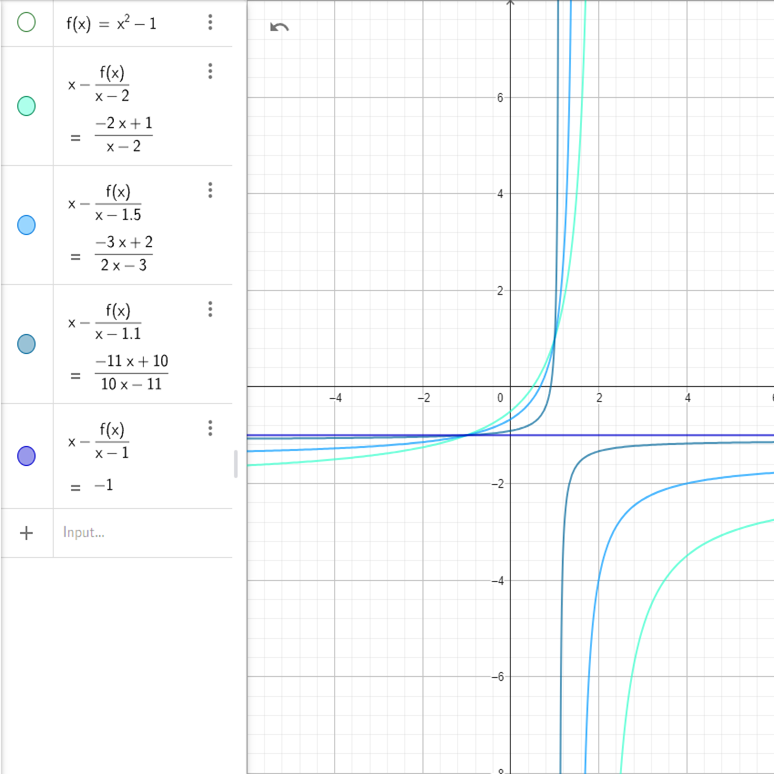
\includegraphics[scale=.6]{./BeispielHerleitung.png}
    %TODO
    \caption{Beispiel:}
\end{figure}\\
%-------------------------------------------------------------------------------------------------------------------
Dabei sieht man, dass es sich, wenn die restlichen Nullstellen nicht genau sind, um eine gebrochen rationale Funktion handelt. Das kann auch an der Gleichung gesehen werden, da diese, mit ein wenig umstellen, aus einem Polynom geteilt durch ein anderes Polynom besteht:
\begin{align*}
    g(x) = y &= x - \frac{p(x)}{\prod_{j=1;j\neq k}^{n} (x-z_j^{(i)})} \\
    &= \frac{x}{1} - \frac{\prod_{j=1}^{n} (x-z_j^{(i)})}{\prod_{j=1;j\neq k}^{n} (x-z_j^{(i)})} \\
    &= \frac{x \cdot \prod_{j=1;j\neq k}^{n} (x-z_j^{(i)})}{\prod_{j=1;j\neq k}^{n} (x-z_j^{(i)})} - \frac{\prod_{j=1}^{n} (x-z_j^{(i)})}{\prod_{j=1;j\neq k}^{n} (x-z_j^{(i)})} \\
    &= \frac{x \cdot \prod_{j=1;j\neq k}^{n} (x-z_j^{(i)}) - \prod_{j=1}^{n} (x-z_j^{(i)})}{\prod_{j=1;j\neq k}^{n} (x-z_j^{(i)})} \\
\end{align*}
Wenn die restlichen Nullstellen gefunden wurden handelt es sich um eine waagrechte lineare Funktion. Das liegt daran, dass alle linearen Faktoren des Polynoms, außer dem der gesuchten Nullstelle, gefunden wurden und nun von dem Polynom dividiert werden. Dabei bleibt $x-(x+z_k^{(i)})$ über. Die beiden $x$ fallen weg und es bleibt der konstante Wert $z_k^{(i)}$ über. Daraus folgt, dass die Funktion waagrecht zu der x-Achse ist.
%-------------------------------------------------------------------------------------------------------------------
\paragraph{Bedeuteung für die Weierstraß-Iteration}
Das Annähern an eine Nullstelle mit jeder Iteration kann man sich mit zwei miteinander verknüpften Annährungen vorstellen. Einerseits das Annähern an die Nullstelle mit der jeweiligen Gleichung für die Nullstelle und andererseits das Annähren der Funktion g(x) an die Waagrechte $y=z_k$, mit immer Genaueren restlichen Nullstellen.

\paragraph{Annährung an die Waagrechte $y=z_k$}
Wie in der Abbildung zuvor zu sehen nährt sich die Funktion mit genaueren Nullstellen an die Funktion $y=z_k$ an. Das hat zur Folge, dass die einzelnen Schritte der Weierstraß-Iteration schneller genau werden. Dabei dient die Annährung an $y=z_k$, da die Gleichung, statt der Nullstelle, genauer wird, mehr als Beschleunigung der Methode, während das Annähren an die Nullstelle mithilfe der Gleichung die eigendliche Annährung bringt.

\paragraph{Annähern an die Nullstelle mithilfe der Gleichung}
Für jedes $z_k^{(i)}$, welches weit genug von den Definitionslücken entfernt ist, gilt, dass $g(z_k^{(i)})$ näher an $z_k$ als $z_k^{(i)}$ ist.\\\\
%-------------------------------------------------------------------------------------------------------------------
Für die Herleitung diese Aussage muss zuerst gezeigt werden, dass $g(x)$ eine waagrechte Asymptote besitzt. Dafür kann man sich die zuvor hergeleitete Gleichung
\begin{equation*}
    g(x) = y = \frac{x \cdot \prod_{j=1;j\neq k}^{n} (x-z_j^{(i)}) - \prod_{j=1}^{n} (x-z_j^{(i)})}{\prod_{j=1;j\neq k}^{n} (x-z_j^{(i)})}
\end{equation*}
angucken. Da die Polynome im Zähler normiert und vom gleichen Grad sind, besitzen beide den Term $a_nx^n$ mit $a_n = 1$. Werden diese Polynome nun miteinander subtrahiert, fällt dieser $n$te-Term weg, da er bei beiden Polynomen gleich ist. Somit ist der Grad des Differenzpolynoms $n-1$. \\
\begin{equation*}
    g(x) = y = \frac{\text{Polynom vom Grad }n-1}{\text{Polynom vom Grad }n-1}
\end{equation*}
Da der Nenner und Zähler den gleichen Grad haben hat $g(x)$ eine waagrechte Asymptote\footnote{
    vgl. studimup.de: Asymptoten berechnen und erkennen, URL: \url{https://www.studimup.de/abitur/analysis/asymptoten/#waagerecht} (Zuletzt eingesehen am 04.11.2023) \label{ftn:studimup.de}
}.\\\\
%-------------------------------------------------------------------------------------------------------------------
Wegen dieser waagrechten Asymptote ist $|g(x)|<|x|$ für jedes $x \in \mathbb{R}$ mit ausreichendem Abstand zu den Definitionslücken wahr. Außerdem ist $|g(x)|>|g(z_k)| \land (g(x) \text{ hat das gleiche Vorzeichen wie } z_k)$ für jedes $x \in \mathbb{R}$ mit den gleichen Bedingungen wie zuvor wahr.
Das kann man an der Lage der waagrechten Asymptote sehen. Diese kann man ausrechnen, indem man die Faktoren vor der höchsten Potenz im Zähler durch den Faktor der höchsten Potenz im Nenner teilt\footref{ftn:studimup.de}. Da das Nennerpolynom normiert ist, ist die waagrechte Asymptote gleich des Faktors vor der höchsten Potenz im Zähler. Der Betrag dieser ist größer als $|z_k|$ und hat das gleiche Vorzeichen wie $z_k$.
Daraus folgt, dass jedes $z_k^{(i)}$, welches weit genug von den Definitionslücken entfernt ist, in $g(x)$ eingesetzt einen Wert, welcher näher an $z_k$ als $z_k^{(i)}$ ist, zurückgibt.

\paragraph{Schluss}
Das bedeutet für die Weierstraß-Iteration, dass in den meisten Fällen mit jeder Iteration $z_k^{(i+1)}$ näher an $z_k$ als $z_k^{(i)}$ ist. Außerdem wird in den meisten Fällen mit jeder Iteration $g(x)$ genauer. Da an $z_k$ $g(z_k) = z_k$ ist und mit einem höheren $i$ $z_k^{(i)}$ meist genauer wird, konvergiert die Weierstraß-Iteration meistens. In dem Abschnitt Probleme und Einschränkungen wird mehr auf die Fälle eingegangen, bei denen die Weierstraß-Iteration nicht konvergiert.

\subsubsection{Wählen der Startpunkte}
Alle Nullstellen einer Polynomfunktion befinden sich auf der abgeschlossen Kreisscheibe  $B(0,M) := \{x \in \mathbb{C} \bigr| |x| \le M\}$ mit $M := 1 + \max\{\frac{|a_j|}{|a_n|}\bigr|\text{\space}j=0,\dots,n-1\}$.\footnote{vgl. \glqq\textit{Sei $P(z) = a_nz^n+a_{n-1}z^{n-1}+\dots+a_1z+a_0$ ein komplexes Polynom vom Grad $n \ge 1$. Dann liegen alle Nullstellen von $P(z)$ in der abgeschlossenen Kreisscheibe $B(0,M) := \{z \in \mathbb{C} \bigr| |z| \le M\}$, wobei $M := 1 + \max\{\frac{|a_j|}{|a_n|}\bigr|\text{\space}j=0,\dots,n-1\}$.}\grqq\space Humboldt-Universität zu Berlin: Helga Baum: Nullstellen komplexer Polynome: 6.3. Erster Satz von Cauchy, URL: \url{https://didaktik.mathematik.hu-berlin.de/user/fehlingerl/Helga.pdf} (Zuletzt eingesehen am 30.10.2023)}  Um möglichst genaue Startpunkte zu bekommen kann man diese auf einer Kreislinie innerhalb der Kreisscheibe anordnen. \\
Dabei gibt es keinen \glqq besten\grqq\space Standart für das Wählen des Radius. Jeder Radius ist für manche Funktionen näher und andere weiter von den Nullstellen entfernt. Je nach den Anforderungen kann man einen eigenen Radius für die Kreislinie nehmen. In meiner Implementierung habe ich mich deshalb für $r = |\frac{na_0}{2a_1}| + |\frac{a_{n-1}}{2n}|$ entschieden.\footref{ftn:OscarVilez,5:40}
Dieser Radius ist relativ ressourcensparend und einfach zu implementieren. Jedoch kann auch ein anderer Radius gewählt werden.

%------------------------------------------------------------------------------------
\subsection{Probleme und Einschränkungen}
Die Weierstraß-Iteration hat, neben dem Vorteil, dass sie einfach zu implementieren ist mehrere Nachteile. Auf diese wird im Folgenden eingegangen.
\subsubsection{Normiertes Polynom}
Für die Weierstraß-Iteration muss die gegebene Funktion $p(x)$ in der Form $\prod_{i=1}^n (x-z_i)$ dargestellt werden können. Da $\prod_{i=1}^n (x-z_i)$ ausmultipliziert, in jedem Fall ein normiertes Polynom ergibt, muss $p(x)$ für die Weierstraß-Iteration ein normiertes Polynom sein.
Ist dies nicht der Fall, wird es unmöglich, $p(x)$ in der Form $\prod_{i=1}^n (x-z_i)$ darzustellen. Daraus folgt, dass man die Methode ohne Umwege nicht ausführen kann. \\
Allerdings gibt es eine einfache Lösung für dieses Problem. Wenn man eine Funktion gleich Null setzt, kann man beide Seiten mit einer beliebigen Zahl multiplizieren. Dabei verändert sich das Ergebnis nicht, da $0m = 0$ \space $\forall m \in \mathbb{C}$ ist. Daraus folgt, dass sich die Nullstellen eines Polynoms, wenn dieses mit einer beliebigen Zahl multipliziert wird, nicht verändern. \\
Somit kann man das Polynom, dessen Nullstellen man finden möchte, durch $a_n$ teilen und bekommt ein normiertes Polynom mit den gleichen Nullstellen. Mit diesem kann man dann die Weierstraß-Iteration durchführen.

\subsubsection{Keine generelle Konvergenz}
Die Weierstraß-Iteration ist nicht generell Konvergent. Das bedeutet, dass für bestimmte Startpunkte mancher Polynomfunktionen die Methode gegen Unendlich keinen festen Wert anstrebt. Dabei verfängt sich die Weierstraß-Iteration in periodischen Zyklen\footnote{d. h. die Weierstraß-Iteration wiederholt sich immer wieder in dem gleichen Abstand.}. Es ist nicht generell bestimmt, bei welchen Startpunkten und Polynomen die Weierstraß-Iteration nicht konvergiert. Beispielsweise hat das Polynom $x^3+x+177$ eine offene Menge an Startpunkten, bei denen die Weierstraß-Iteration nicht konvergiert. Da dies allerdings, besonders wenn man vernünftige Startpunkte wählt, sehr selten ist kann es meist vernachlässigt werden. 

\section{Implementierung}
\subsection{Einleitung}
Im Folgenden wird auf die Implementierung der Weierstraß-Iteration in Java eingegangen. Dabei wurde die Weierstraß-Iteration in der Klasse \glqq Weierstrass\grqq\space implementiert. Neben dieser Klasse wurden zwei Klassen \glqq Poly\grqq\space und \glqq Complex\grqq\space erstellt. Diese haben die Funktion Polynomfunktionen und komplexe Zahlen darzustellen. In der Klasse \glqq Weierstrass\grqq\space befindet sich der \glqq Entry-Point\grqq\space bzw. die \glqq main\grqq-Methode des Programmes.

\subsection{Komplexe Zahlen}
In Java gibt es keinen eingebauten Weg mit komplexen Zahlen zu rechnen. Es ist möglich mithilfe einer Bibliothek komplexe Zahlen zu nutzen, jedoch ist es nicht gegeben, dass alle nötigen Operationen eingebaut sind. Deshalb habe ich mich dazu entschieden eine eigene Klasse \glqq Complex\grqq\space zu schreiben, um volle Kontrolle über die Methoden und Implementierung der komplexen Zahlen zu haben.

\subsubsection{Attribute}
Die Attribute \glqq real\grqq\space und \glqq imaginary\grqq\space repräsentieren den reellen und imaginären Teil der komplexen Zahl.

\subsubsection{Konstruktor}
\paragraph{Complex(double real, double imaginary)} 
Initialisiert eine komplexe Zahl mit einem gegebenen Real- und Imaginärteil.

\subsubsection{Methoden}
\paragraph{public double abs()} 
Berechnet und gibt den Betrag der komplexen Zahl zurück.

\paragraph{public Complex round(int accuracyDecimalPlaces)} 
Rundet den Real- und Imaginärteil auf die angegebene Anzahl von Dezimalstellen und gibt eine neue komplexe Zahl zurück.

\paragraph{@Override public String toString()} 
Gibt eine lesbare Repräsentation der komplexen Zahl als String zurück.

\subsubsection{Statische Methoden}
Die statischen Methoden führen grundlegende Rechenoperationen Addition, Subtraktion, Multiplikation, Division und Potenzierung mit komplexen Zahlen durch.

%-----------------------------------------------------------------------------------------
\subsection{Polynomfunktion}
Polynomfunktionen werden mit der Klasse \glqq Poly\grqq\space dargestellt. 

\subsubsection{Attribute}
In dem Array \glqq coefficients\grqq\space von Gleitkommazahlen (double) sind die Koeffizienten des Polynoms enthält. Der Index repräsentiert den Exponenten des zugehörigen Terms.
Der Grad des Polynoms wird als Integer in dem Attribut \glqq degree\grqq\space gespeichert. 

\subsubsection{Konstruktor}
Der Konstruktor \glqq Poly(double... coefficients)\grqq, erstellt ein Polynom mit den gegebenen Koeffizienten.

\subsubsection{Methoden}
\paragraph{public void normalise()} 
Eine Methode, die das Polynom für die Weierstraß-Iteration normiert. Hierbei wird jeder Koeffizient durch den führenden Koeffizienten $a_n$ des Polynoms geteilt. Die Nullstellen des Polynoms ändern sich nicht, aber die Darstellung des Polynoms ändert sich.

\paragraph{public Complex solve(Complex val)}
Eine Methode, die den Funktionswert des Polynoms für einen gegebenen komplexen Wert \glqq val\grqq\space berechnet. Dabei wird das Horner-Schema\footnote{
    Das Horner-Schema ist eine effiziente Methode zur Berechnung des Funktionswerts eines Polynoms. Es erfolgt eine schrittweise Auswertung, bei der jeder Term des Polynoms mit dem $x$-Wert multipliziert und mit dem vorherigen Ergebnis addiert wird, wodurch der Rechenaufwand minimiert wird.
} verwendet, um die Auswertung effizient durchzuführen. 

\paragraph{@Override public String toString()}
Die \glqq toString()\grqq -Methode wurde überschrieben, um eine lesbare Darstellung des Polynoms auszugeben. Die Methode berücksichtigt verschiedene Fälle, einschließlich der Anzeige von Termen mit positiven oder negativen Koeffizienten und der Auslassung von Termen mit Koeffizienten gleich null.

%----------------------------------------------------------------------------------------------------------
\subsection{Weierstraß-Iteration}

\subsubsection{calc(Poly p, Complex[] roots, int index)}
Die \glqq calc-Methode\grqq\space berechnet die nächste Iteration für eine NUllstelle des Polynoms unter Verwendung der Weierstraß-Iterationsformel. Dabei werden drei Parameter entgegengenommen: das Polynom \glqq p\grqq, für das die Nullstellen berechnet werden, ein Array von komplexen Zahlen \glqq roots\grqq, das die aktuellen Näherungen der Nullstellen enthält und der Index der Nullstelle, die in dieser Iteration aktualisiert wird.\\
Für die Berechnung werden zunächst der Zähler (\glqq numerator\grqq) und der Nenner (\glqq denominator\grqq) des Weierstrass-Korrekturterms berechnet. Dann wird dieser Korrekturterm von der aktuellen Nullstelle subtrahiert, um die nächste Näherung zu erhalten.

\subsubsection{startingPoints(Poly p, int accuracyDecimalPlaces)}
Die \glqq startingPoints\grqq-Methode generiert anhand der Eigenschaften des Polynoms anfängliche Schätzungen für die Nullstellen. Sie nimmt als Parameter das Polynom \glqq p\grqq\space entgegen und gibt ein Array von komplexen Zahlen zurück, das die initialen Schätzungen der Nullstellen enthält.\\
Die Methode verwendet die zuvor beschreibenen Berechnungen, um den Radius und den Winkel für die Platzierung der Anfangsschätzungen auf einem Kreis in der komplexen Ebene zu bestimmen. Die generierten Startpunkte werden als Ausgangspunkte für die Weierstraß-Iteration verwendet.

\subsubsection{isAccurateEnough(Complex[] newRoots, Complex[] oldRoots, double accuracy)}
Die \glqq isAccurateEnough\grqq-Methode überprüft, ob die Nullstellen ausreichend genau konvergiert sind. Sie vergleicht den Unterschied zwischen den neuen Nullstellen und den alten Nullstellen mit einer vorgegebenen Genauigkeitsgrenze (accuracy).\\
Die Methode gibt Wahr zurück, wenn alle Nullstellen innerhalb der Genauigkeitsgrenze konvergiert sind, andernfalls gibt sie Falsch zurück.

\subsubsection{weierstrass(Poly p)}
Die \glqq Weierstrass\grqq-Methode ist die Hauptmethode der Weierstraß-Iteration. Sie nimmt ein Polynom entgegen und gibt ein Array von komplexen Zahlen mit Nährungen der Nullstellen des Polynoms zurück. Die Methode kann in sechs Schritte unterteilt werden.

\paragraph{1. Polynom normieren}
Zuerst wird das Polynom normiert, um die Weierstraß-Iteration möglich zu machen. Dafür wird die Methode \glqq normalise()\grqq\space der Polynomfunktion aufgerufen.

\paragraph{2. Genauigkeit und maximale Iterationen festlegen}
Darauffolgend wird die Genauigkeit mit $10^{-4}$ und maximale Anzahl an Iterationen mit $1000$ festgelegt.

\paragraph{3. Initialisierung der Nullstellen}
Als nächstes werden mithilfe der zuvor behandelten Funktion \glqq startingPoints(Poly p)\grqq\space die Nullstellen in einem Array Initialisiert.

\paragraph{4. Durchführen der Weierstraß-Iteration}
Jetzt kann eine Schleife gestartet werden, die solange läuft, bis die Konvergenz erreicht ist oder die maximale Anzahl von Iterationen erreicht ist. In dieser wird die Funktion \glqq calc(Poly p, Complex[] roots, int index)\grqq\space für alle Nullstellen bei jeder Iteration ausgeführt.

\paragraph{5. Probe}
Nach Abschluss der Iteration wird eine Probeausgabe für jede gefundene Wurzel gemacht, um die Genauigkeit zu überprüfen.

\paragraph{6. Rückgabe der Nährungen der Nullstellen}
Zuletzt wird das endgültige Array der berechneten Wurzeln zurückgegeben.

\subsection{Input/Output}
Der Input erfolgt mithilfe der Bibliothek \glqq java.util.Scanner\grqq\space in der \glqq main\grqq-Methode. Dabei wird für jeden Term des Polynoms nach dem Koeffizienten gefragt. Es wird bei dem $0$ten Term begonnen und in aufsteigender Reihenfolge weitergefragt. Wenn der gewünschte Grad erreicht ist kann der Nutzer \glqq done\grqq\space eingeben und die Weierstraß-Iteration wird mit dem gegebenen Polynom ausgeführt.\\
\\
Darauffolgend wird zuerst die Polynomfunktion zur Kontrolle ausgegeben. Während die Weierstraß-Iteration ausgeführt wird werden alle Nährungen an die Nullstellen für diese Iteration angegeben. Zuletzt wird das Polynom ein letztes mal ausgegeben und jede der Nullstellen in dieses eingesetzt. Bei diesen sollte, falls die Weierstraß-Iteration funktiontiert hat \glqq 0.0\grqq\space herrauskommen.\footnote{
    %TODO screenshot beispiel
}

%TODO footnote zu jeder Methode

\section{Fazit}
\subsection{Zusammenfassung}
- Man bildet $n$ Gleichungen für $n$ Nullstellen\\
- Man wählt Startpunkte\\
- Man iteriert mit den Gleichungen, bis Endkriterium erreicht ist\\
- Findet Nullstellen

\subsection{Bezug zu der Problemstellung}
- Jetzt weiß man, wie man Nullstellen numerisch findet\\
- Damit kann man das und dass machen

\subsection{Wieso die Weierstraß-Iteration?}
- Weierstraß deswegen gewählt\\
- Bessere Verfahren, jedoch Weierstraß-Iteration relativ verständlich (Nicht mit extrem komplexen mathematischen Konstrukten)

\subsection{Reflektion}
- Manche dinge nicht vollkommen hergeleitet, weil diese einzelnen Dinge eine eigene Facharbeit bräuchten\\
- Der richtige Beweis ist einfach zu komplex für ein Unterthema in einer Facharbeit.

\end{document}